\documentclass[14pt,a4paper,report]{report}
\usepackage[a4paper, mag=1000, left=2.5cm, right=1cm, top=2cm, bottom=2cm, headsep=0.7cm, footskip=1cm]{geometry}
\usepackage[utf8]{inputenc}
\usepackage[english,russian]{babel}
\usepackage{indentfirst}
\usepackage[dvipsnames]{xcolor}
\usepackage[colorlinks]{hyperref}
\usepackage{listings} 
\usepackage{fancyhdr}
\usepackage{caption}
\usepackage{graphicx}
\hypersetup{
	colorlinks = true,
	linkcolor  = black
}

\usepackage{titlesec}
\titleformat{\chapter}
{\Large\bfseries} % format
{}                % label
{0pt}             % sep
{\huge}           % before-code


\DeclareCaptionFont{white}{\color{white}} 

% Listing description
\usepackage{listings} 
\DeclareCaptionFormat{listing}{\colorbox{gray}{\parbox{\textwidth}{#1#2#3}}}
\captionsetup[lstlisting]{format=listing,labelfont=white,textfont=white}
\lstset{ 
	% Listing settings
	inputencoding = utf8,			
	extendedchars = \true, 
	keepspaces = true, 			  	 % Поддержка кириллицы и пробелов в комментариях
	language = C,            	 	 % Язык программирования (для подсветки)
	basicstyle = \small\sffamily, 	 % Размер и начертание шрифта для подсветки кода
	numbers = left,               	 % Где поставить нумерацию строк (слева\справа)
	numberstyle = \tiny,          	 % Размер шрифта для номеров строк
	stepnumber = 1,               	 % Размер шага между двумя номерами строк
	numbersep = 5pt,              	 % Как далеко отстоят номера строк от подсвечиваемого кода
	backgroundcolor = \color{white}, % Цвет фона подсветки - используем \usepackage{color}
	showspaces = false,           	 % Показывать или нет пробелы специальными отступами
	showstringspaces = false,    	 % Показывать или нет пробелы в строках
	showtabs = false,           	 % Показывать или нет табуляцию в строках
	frame = single,              	 % Рисовать рамку вокруг кода
	tabsize = 2,                  	 % Размер табуляции по умолчанию равен 2 пробелам
	captionpos = t,             	 % Позиция заголовка вверху [t] или внизу [b] 
	breaklines = true,           	 % Автоматически переносить строки (да\нет)
	breakatwhitespace = false,   	 % Переносить строки только если есть пробел
	escapeinside = {\%*}{*)}      	 % Если нужно добавить комментарии в коде
}

\begin{document}

\def\contentsname{Содержание}

% Titlepage
\begin{titlepage}
	\begin{center}
		\textsc{ФЕДЕРАЛЬНОЕ ГОСУДАРСТВЕННОЕ АВТОНОМНОЕ ОБРАЗОВАТЕЛЬНОЕ УЧРЕЖДЕНИЕ ВЫСШЕГО ОБРАЗОВАНИЯ
«САНКТ-ПЕТЕРБУРГСКИЙ ПОЛИТЕХНИЧЕСКИЙ УНИВЕРСИТЕТ ПЕТРА ВЕЛИКОГО»\\[5mm]
			Институт компьютерных наук и технологий\\
			Высшая школа интеллектуальных систем и суперкомпьютерных технологий}
		
		\vfill
		
		\textbf{Дисциплина «Цифровые ресурсы в научных исследованиях»\\[10mm]
		ОТЧЕТ\\[2mm]
		по практической работе №2\\[2mm]
		на тему\\[2mm]
			«Поиск источников научной и образовательной информации в Интернет и с использованием сервисов дискавери»\\[41mm]
		}
	\end{center}
	
	\hfill
	\begin{minipage}{.4\textwidth}
		Выполнил:\\[2mm] 
        Студент группы 3540901/02001\\
		Дроздов Н.Д.\\[2mm]
        «....» ................... 2020г., ...............\\
        \hspace*{38mm} (Подпись)\\[2mm]
		Проверил:\\[2mm] 
		Бендерская Е.Н.\\[2mm]
		«....» ................... 2020г., ...............\\
        \hspace*{38mm} (Подпись)\\
	\end{minipage}
	\vfill
	\begin{center}
		Санкт-Петербург\\ \the\year\ г.
	\end{center}
\end{titlepage}

% Contents
\tableofcontents
\clearpage

\chapter{Практическая работа №2}

\section{Цель работы}

Сформировать знания по поиску и отбору информации в различных поисковых системах

\section{Задачи}

\begin{enumerate}
	
	\item Изучить методику поиска информации.
	
	\item Получить навыки поиска информации в различных информационно-поисковых системах.
	
\end{enumerate}

\clearpage

\section{Ход работы}

\subsection{Задание 1}

\subsubsection{Найти актуальную литературу по блокчейну для написания обзора.}

\begin{enumerate}
	
	\item Выполняем поиск с помощью одной из информационных систем глобальной сети (например, Google) . Результат поиска – 5 750 000;
	
	\item Сортируем по фильтру «Книги». Результат – 13 300;
	\begin{figure}[h!]
    \centering
    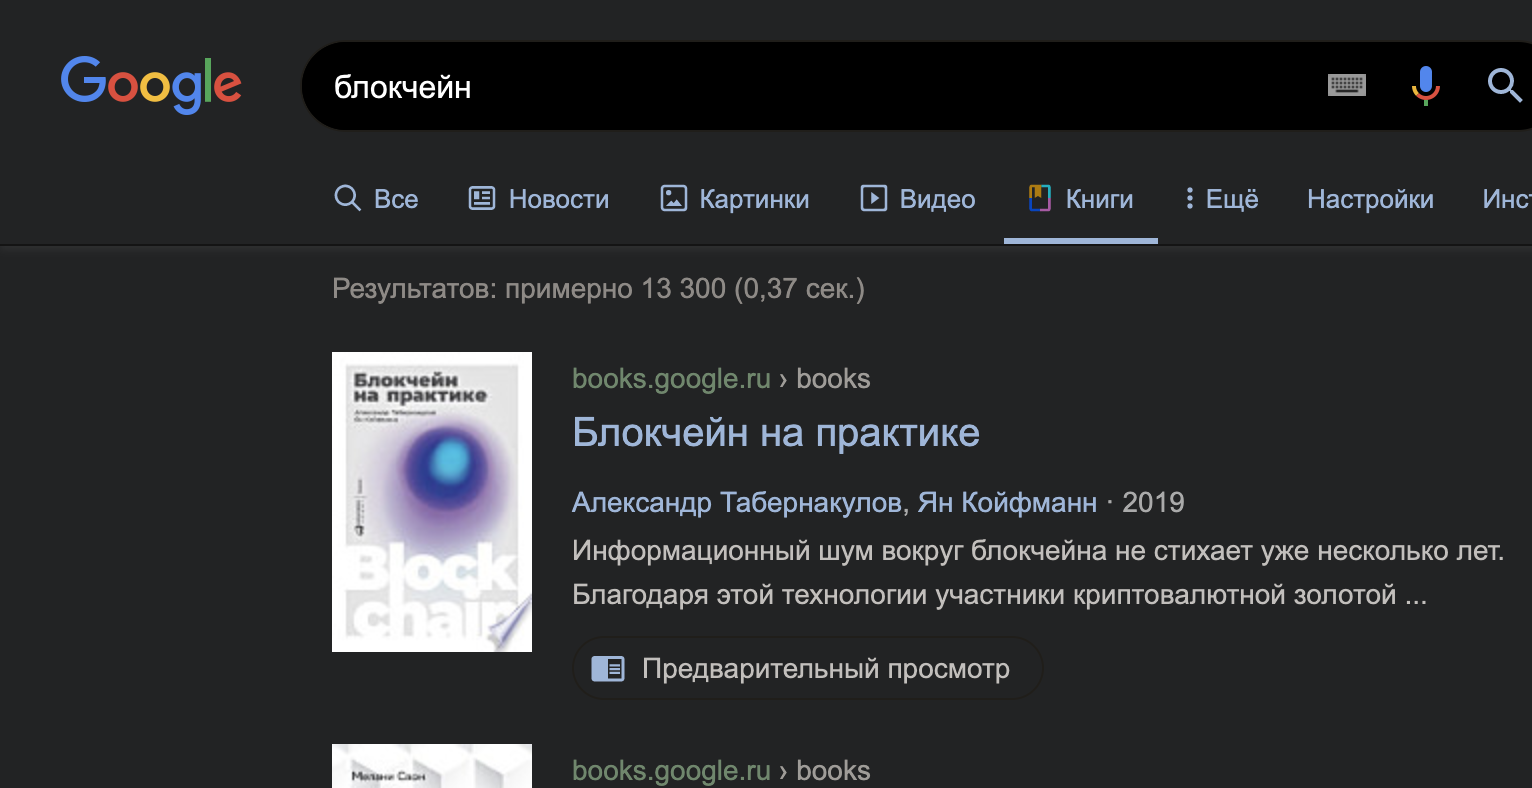
\includegraphics[scale = 0.33]{1.png}
    \caption{Результаты поиска в поисковой системе Google.}
    \label{image:1}
    \end{figure}
    
    \item Выполняем поиск в зарубежных БД с использованием сервисов дискавери, для чего вводим искомое слово на русском и английском языках. Найдено 5483 ресурсов
	\begin{figure}[h!]
    \centering
    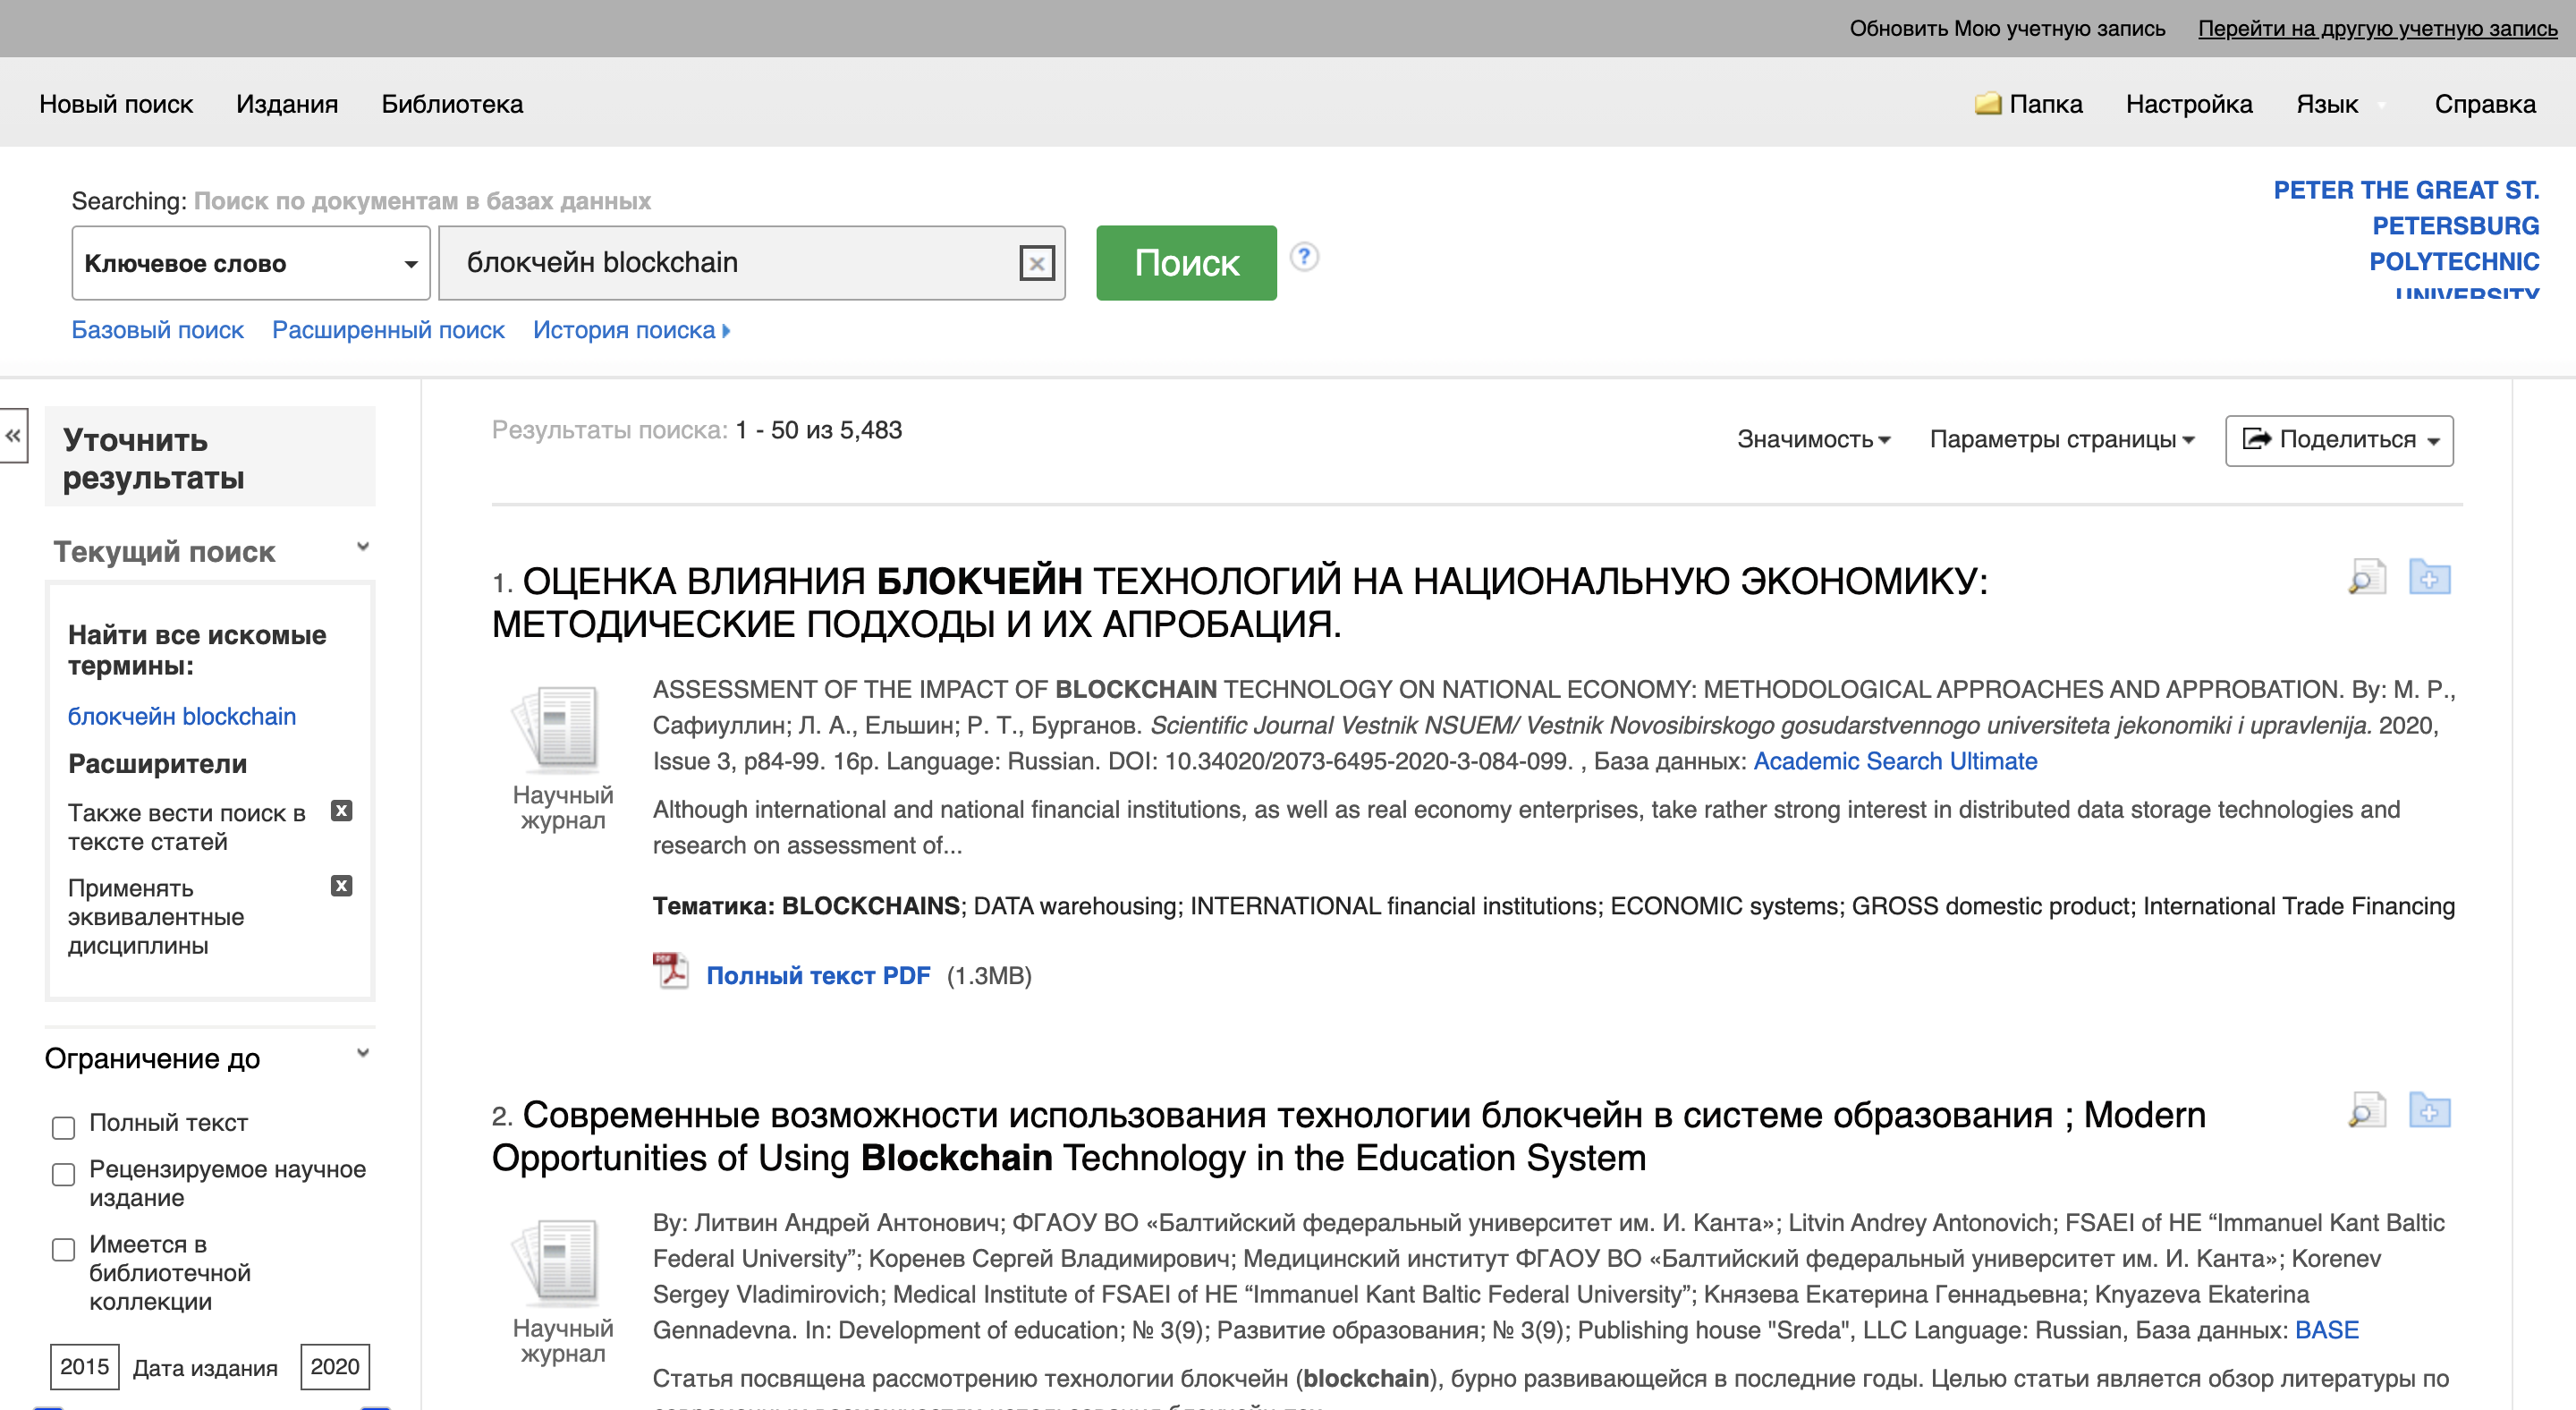
\includegraphics[scale = 0.33]{2.png}
    \caption{Результаты поиска по ресурсам зарубежных баз.}
    \label{image:1}
    \end{figure}
    
    \clearpage
    
    Виды источников:
	\begin{figure}[h!]
    \centering
    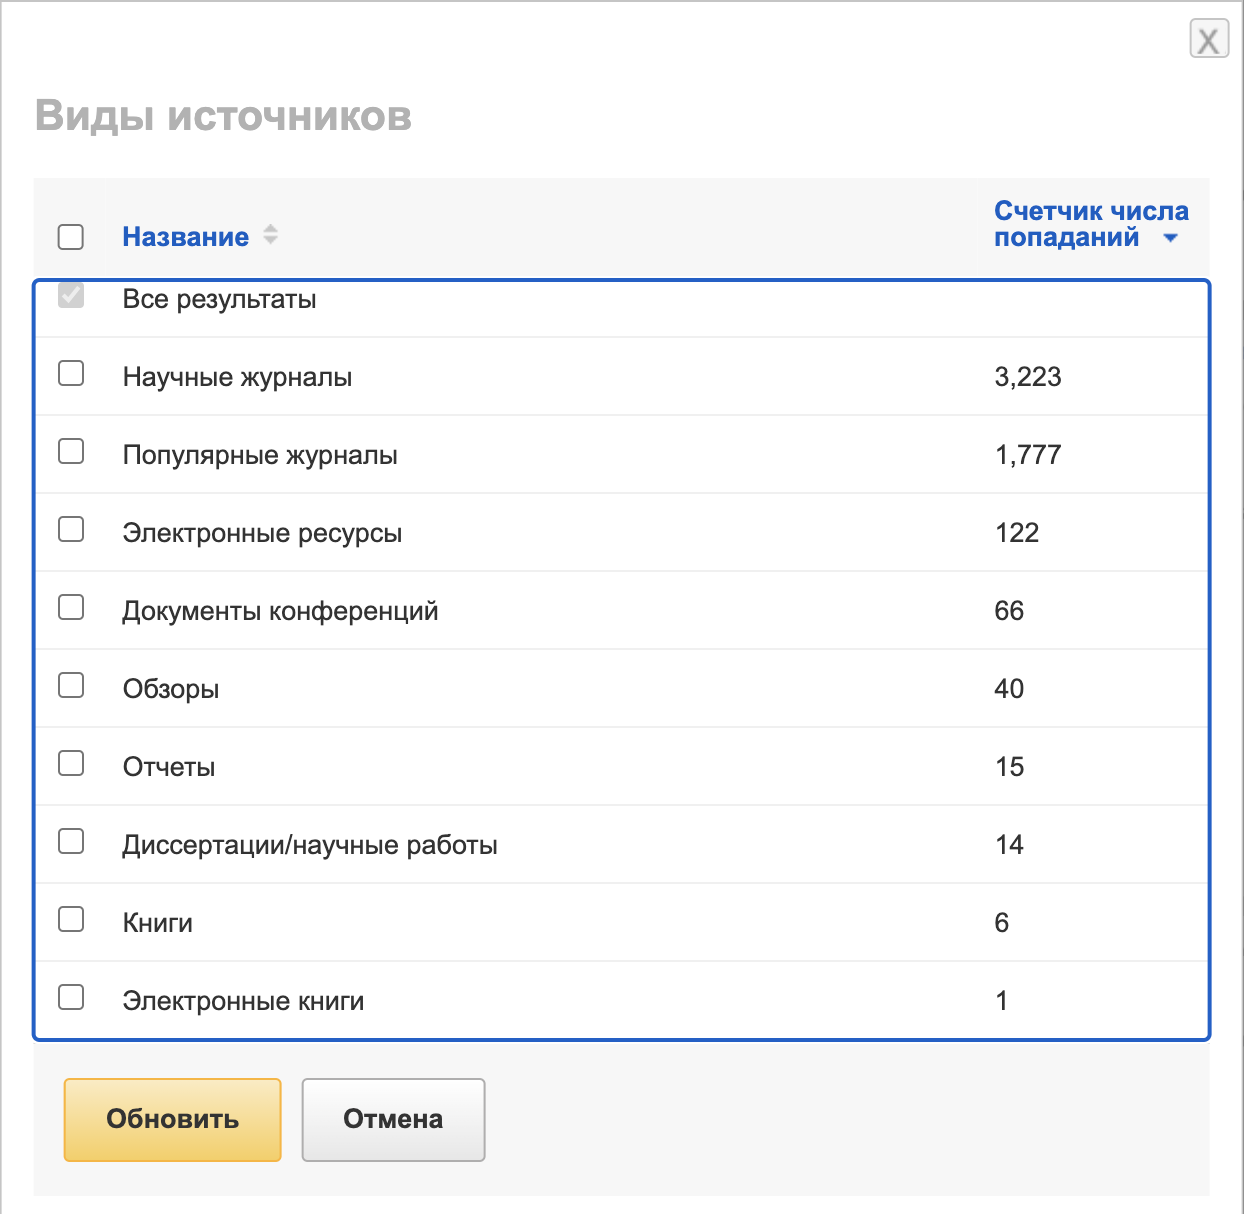
\includegraphics[scale = 0.33]{3.png}
    \caption{Виды источников.}
    \label{image:1}
    \end{figure}
    
    \item Шаг 3-4. Оцениваем результаты. Найдены несколько тысяч ресурсов, доступ к некоторым может быть получен мгновенно из Интернет, также часть ресурс требует заказа на абонементе библиотеки, остальные могут быть заказаны в отделе МБА/ЭДД. Сразу же можно составить список актуальной литературы по заданной теме (все издания – после 2015 г.).
    
	
\end{enumerate}



\section{Вывод}
В ходе проделанной практической работы были получены навыки и умения ориентирования в информационных ресурсах различных поисковых систем, правильно формировать поисковые запросы, самостоятельно осуществлять поиск необходимой библиографической информации, пользоваться предлагаемыми инструментами для сокращения результатов поисковых запросов.
\clearpage

\end{document}